\documentclass[tikz, border=2pt]{standalone}
\usepackage{amsmath}

\begin{document}
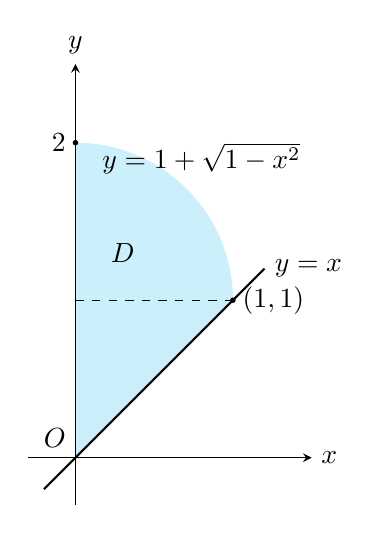
\begin{tikzpicture}[scale=2, >=stealth]
    % 填充积分区域 D
    % 区域顶点：(0,0), (0,2), (1,1)
    % 填充路径：从 (0,0) 沿 y 轴到 (0,2)，然后沿圆弧到 (1,1)，再沿直线 y=x 回到 (0,0)
    \fill[cyan!20] (0,0) -- (0,2) arc (90:0:1) -- cycle; % 弧的起点是 (0,2) 对应角度90，终点是 (1,1) 对应角度0

    % 画坐标轴
    \draw[->] (-0.3, 0) -- (1.5, 0) node[right] {$x$};
    \draw[->] (0, -0.3) -- (0, 2.5) node[above] {$y$};

    % 画直线 y=x
    \draw[thick] (-0.2, -0.2) -- (1.2, 1.2) node[right] {$y=x$};

    \draw[dashed, thin] (0, 1) -- (1, 1);

    % 画圆弧 y = 1 + sqrt(1-x^2) (即 x^2 + (y-1)^2 = 1 的上半部分)
    % 圆心 (0,1), 半径 1

    % 标注关键点
    \node[above left] at (0,0) {$O$};
    \fill (0,2) circle (0.5pt) node[left] {$2$};
    \fill (1,1) circle (0.5pt) node[right] {$(1,1)$};

    % 标注区域 D
    \node at (0.3, 1.3) {$D$};
    \node at (0.8, 1.9) {$y=1+\sqrt{1-x^2}$};
\end{tikzpicture}
\end{document}
